
\begin{wrapfigure}{r}{0.5\textwidth}
  \begin{center}
    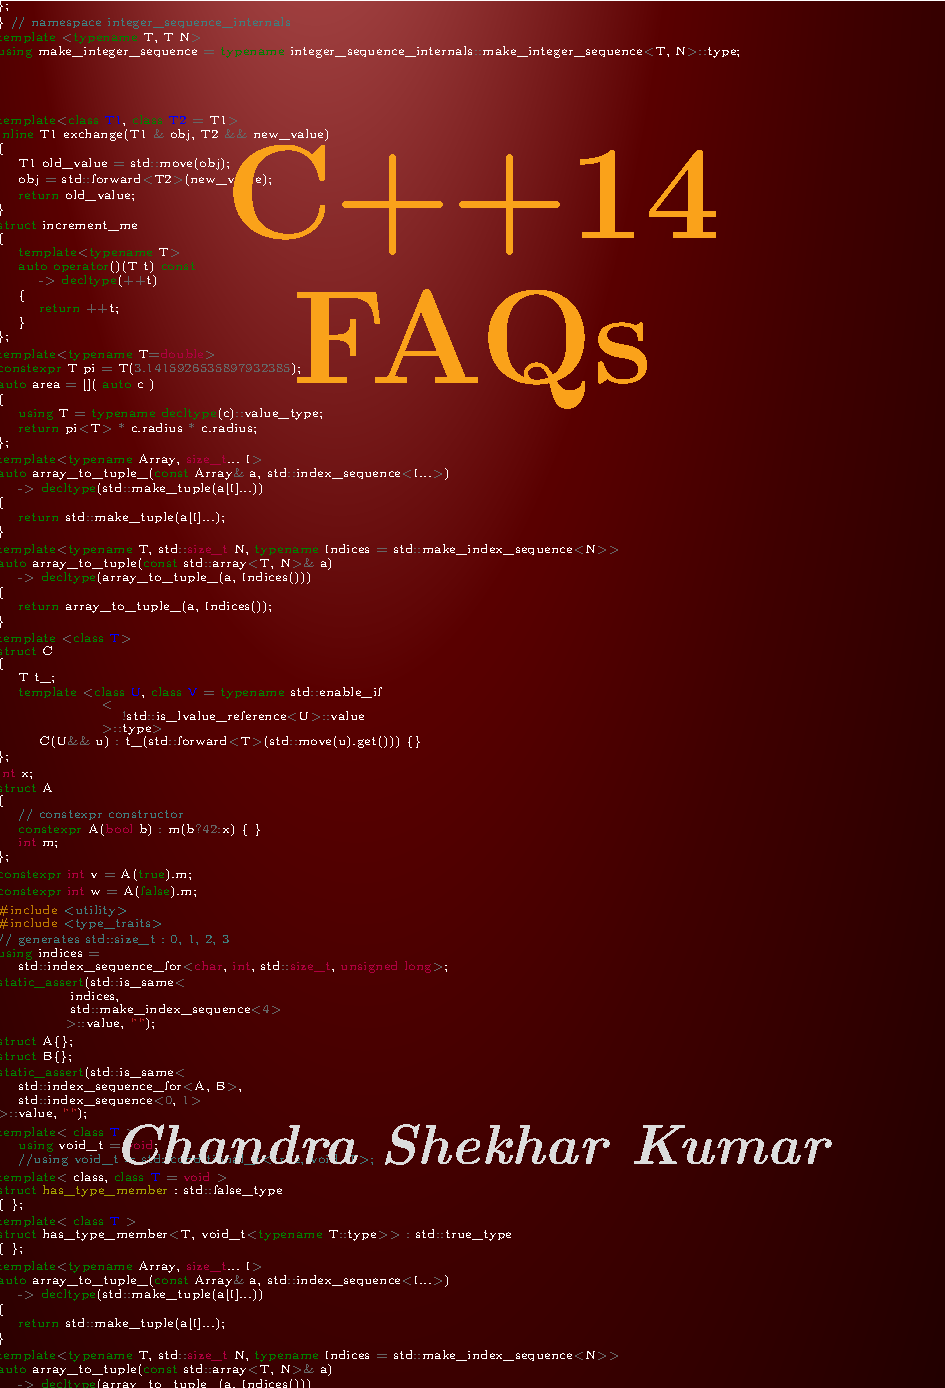
\includegraphics[width=0.5\textwidth]{cpp14faqs/cover}
  \end{center}
  %\caption{Front Cover}
\end{wrapfigure}

This book contains selected questions (84) related to C++14 with detailed solutions to all of these which will help the reader to hone her skills to solve a particular problem.

Primary source of this collection is \emph{Advanced C++ FAQs: Volumes 1 \& 2}.

This book is not an introduction to C++. It assumes that the reader is aware of the basics of C++98 and C++03 and wants to expand her horizon to latest and greatest in C++14(aka C++1y). The problems are marked on a scale of one(*)(simplest) to five stars(*****)(hardest).

\hrulefill

\underline{\textbf{\textcolor{BurntOrange}{Excerpt} \textcolor{Sepia}{(Questions 1-23 with Solutions):}}}

\section{variable templates}


\begin{Exercise}[title={variable template}, difficulty=3, label=ex01]
\index{variable template}
What is a \emph{variable template} ?
\end{Exercise}



\begin{Answer}[ref=ex01]\index{variable template}
A \emph{variable template} is a declaration which is introduced by a template declaration of a variable. As we already know that a template declaration is also a definition if its declaration defines a function, a class, a variable, or a static data member.

A \emph{variable template} at class scope is a \emph{static data member template}.

Consider a simple template meta function, which uses variable template feature to store the boolean value of result of comparing two types:
\begin{lstlisting}
template <typename T, typename U>
constexpr bool is_same = std::is_same<T, U>::value;

bool t = is_same<int, int>; // true
bool f = is_same<int, float>; // false
\end{lstlisting}

The types of variable templates are not restricted to just built-in types; they can be user defined types.
\begin{lstlisting}
struct matrix_constants 
{
    template<typename T>
    using pauli = hermitian_matrix<T, 2>;
    
    template<typename T>
    constexpr pauli<T> sigma1 = { { 0, 1 }, { 1, 0 } };

    template<typename T>
    constexpr pauli<T> sigma2 = { { 0, -1i }, { 1i, 0 } };

    template<typename T>
    constexpr pauli<T> sigma3 = { { 1, 0 }, { -1, 0 } };
};
\end{lstlisting}

It makes definitions and uses of parameterized constants much simpler, leading to
simplified and more uniform programming rules to teach and to remember like:
\begin{lstlisting}
template<typename T>
struct lexical_cast_fn
{
    template<typename U>
    T operator()(U const &u) const
    {
        //...
    }
};

template<typename T>
constexpr lexical_cast_fn<T> lexical_cast{};

int main()
{
    lexical_cast<int>("42");
}
\end{lstlisting}

\end{Answer}



\section{Constexpr static data members of class templates}

\begin{Exercise}[title={\small Constexpr static data members of class templates}, difficulty=3, label=ex02]
\index{Constexpr static data members of class templates}
What is issue with constexpr static data members of class templates ?
\end{Exercise}


\begin{Answer}[ref=ex02]\index{Constexpr static data members of class templates}
Let us revisit how \emph{std::is\_same} is designed:

\begin{lstlisting}
template<typename T, T v>
struct integral_constant 
{
    static constexpr T value = v;
    typedef T value_type;
    ....
};

template<typename T, T v>
constexpr T integral_constant<T, v>::value;

typedef integral_constant<bool, true>  true_type;
typedef integral_constant<bool, false> false_type;

template<typename T, typename U>
struct is_same : false_type{};

template<typename T>
struct is_same<T, T> : true_type{};
\end{lstlisting}

The main problems with \emph{static data member} are:
\begin{itemize}
    \item they require \emph{duplicate} declarations: 
    \begin{enumerate}
        \item once inside the class template, 
        \item once outside the class template to provide the real definition in case the constants is odr(One Definition Rule) used.
    \end{enumerate}
    \item It creates confusion by the necessity of providing twice the same declaration, whereas ordinary constant declarations do not need duplicate declarations.
\end{itemize}

The standard class \emph{numeric\_limits} also suffers from the same problem as far as constexpr static data members are concerned.

\end{Answer}



\section{constexpr function templates}

\begin{Exercise}[title={constexpr function templates}, difficulty=3, label=ex03]
\index{constexpr function templates}
What is issue with constexpr function templates ?
\end{Exercise}


\begin{Answer}[ref=ex03]\index{constexpr function templates}
Constexpr functions templates provide functional abstraction.

A simple constexpr function template :
\begin{lstlisting}
template <typename T, typename U>
constexpr bool is_same()
{
    return std::is_same<T, U>::value;
}
\end{lstlisting}
Constexpr functions templates  do not have the duplicate declarations issue that static data members have.

However, they force us to chose in advance, at the definition site, how the constants are to be delivered: either by a const reference, or by plain non-reference type. 

If delivered by const reference then the constants must be systematically be allocated in static storage.

If by non-reference type, then the constants need copying. 

Copying isn't an issue for built-in types, but it is an issue for user-defined types with value semantics that aren't just wrappers around tiny built-in types

Whereas ordinary const(expr) variables do not suffer from this problem. A simple definition is provided, and the decision of whether the constants actually needs to be layout out in
storage only depends on the usage, not the definition.

Another examples are the static member functions of \emph{std::numeric\_limits} and functions like $boost::constants::pi<T>()$:
\begin{lstlisting}
#include <boost/math/constants/constants.hpp>

template <class Real>
Real area(Real r)
{
   using namespace boost::math::constants;
   return pi<Real>() * r * r;
}
\end{lstlisting}
The function template versions of the constants are simple inline functions that return a constant of the correct precision for the type used. In addition, these functions are declared constexpr for those compilers that support this, allowing the result to be used in constant expressions provided the template argument is a literal type. 

It looks like we are creating constexpr functions only to return a constant.

\end{Answer}




\section{variable templates in action}

\begin{Exercise}[title={variable templates in action}, difficulty=2, label=ex04]
\index{variable templates}
Illustrate how \emph{variable templates} can be used to compute the area of a circle for a given type with appropriate precision?
\end{Exercise}


\begin{Answer}[ref=ex04]\index{variable templates in action}
\emph{variable templates} address both of the issues illustrated before and no syntax modification was required to incorporate this feature in C++11 because current grammar allows any declaration to be parameterized. It was prohibited earlier via semantic constraints which is relaxed now on template declarations.

Let us first represent the mathematical constant $\pi$ with precision dictated by a floating point datatype:
\lstinputlisting[caption=$\pi$ and variable template]{cpp14faqs/code/c++14/variable_template.cpp}
With the following command:
\begin{verbatim}
clang++ -std=c++1y variable_template.cpp 
\end{verbatim}

we get the following output:
\begin{verbatim}
pi<int> : 3
pi<float> : 3.1415927410125732421875
pi<double> : 3.141592653589793115997963468544185161591
\end{verbatim}

This variable template can be used in a generic function to compute the area of a circle for a given radius:
\lstinputlisting{cpp14faqs/code/c++14/variable_template_area.cpp}

\end{Answer}




\section{static data member template}

\begin{Exercise}[title={static data member template}, difficulty=2, label=ex05]
\index{static data member template}
Provide a suitable definition of the static data member template \emph{min}:
\begin{lstlisting}
struct limits 
{
    template<typename T>
    static const T min; // declaration of min
};
\end{lstlisting}
\end{Exercise}


\begin{Answer}[ref=ex05]\index{static data member template}
As we already know that a variable template at class scope is a \emph{static data member template} and a definition for a static data member or static data member template may be provided in a namespace scope enclosing the definition of the static member's class template. 
\begin{lstlisting}
struct limits 
{
    template<typename T>
    static const T min; // declaration of min
};

template<typename T>
const T limits::min = { }; // definition of min
\end{lstlisting}
\end{Answer}



\section{specialization of variable template}

\begin{Exercise}[title={specialization of variable template}, difficulty=3, label=ex06]
\index{specialization of variable template}
Simplify the program below to do the needful:

\begin{lstlisting}
template <typename T, typename U>
constexpr bool is_same = std::is_same<T, U>::value;

bool t = is_same<int, int>; // true
bool f = is_same<int, float>; // false
\end{lstlisting}

\end{Exercise}


\begin{Answer}[ref=ex06]\index{specialization of variable template}
Variable templates are subject to template specialization like template functions, so we can simplify the code as follows:

\begin{lstlisting}
template<typename T, typename U>
constexpr bool is_same = false;

template<typename T>
constexpr bool is_same<T, T> = true;
\end{lstlisting}
\end{Answer}




\section{default argument and specialization of variable template}

\begin{Exercise}[title={\small default argument and specialization of variable template}, difficulty=3, label=ex07]
\index{default argument and specialization of variable template}
What is the output of the program ?
\lstinputlisting{cpp14faqs/code/c++14/specialize_variable_templates.cpp}

\end{Exercise}


\begin{Answer}[ref=ex07]\index{default argument and specialization of variable template}
\begin{verbatim}
pi<> : 3.14159265358979311599796346854
pi<int> : 3.1415927410125732421875
pi<float> : 3.1415927410125732421875
\end{verbatim}
\end{Answer}





\section{lambda and variable template}

\begin{Exercise}[title={\small lambda and variable template}, difficulty=3, label=ex08]
\index{lambda and variable template}

Simplify the program below.
\lstinputlisting{cpp14faqs/code/c++14/variable_template_area.cpp}

\end{Exercise}


\begin{Answer}[ref=ex08]\index{lambda and variable template}

\lstinputlisting{cpp14faqs/code/c++14/variable_template_simplify.cpp}

\end{Answer}





\section{variable templates variables vary}

\begin{Exercise}[title={variable templates variables vary}, difficulty=2, label=ex09]
\index{variable templates variables vary}

Is this a legal code ? 
\lstinputlisting{cpp14faqs/code/c++14/variable_template1.cpp}

If yes, what is the output ?

\end{Exercise}


\begin{Answer}[ref=ex09]\index{variable templates variables vary}

Yes, the code is correct because variable template instances are first-class objects.

Output is :
\begin{verbatim}
42
0
\end{verbatim}

\end{Answer}





\section{auto variable templates}

\begin{Exercise}[title={variable templates variables vary}, difficulty=2, label=ex010]
\index{auto variable templates}

Is this a legal code ? 
\lstinputlisting{cpp14faqs/code/c++14/auto_variable_templates.cpp}


\end{Exercise}


\begin{Answer}[ref=ex010]\index{auto variable templates}
Yes, a specialization of a variable template is a variable and as per the standard : \emph{No diagnostic shall be issued for a template for which a valid specialization can be generated}.

\end{Answer}





\section{valid specialization but error ?}

\begin{Exercise}[title={valid specialization but error}, difficulty=3, label=ex011]
\index{valid specialization but error}

Why this code doesn't compile ?
\lstinputlisting{cpp14faqs/code/c++14/specialize.cpp}


\end{Exercise}


\begin{Answer}[ref=ex011]\index{valid specialization but error}
Typical error is:
\begin{verbatim}
specialize.cpp:3:17: error: ‘typedef int Y::type’ is private
     typedef int type;
                 ^
specialize.cpp:6:13: error: within this context
 template<Y::type N>
             ^
\end{verbatim}
Because the template parameter declaration is ill-formed, it gets diagnosed immediately and does not form any larger structure. Hence there is no template to be specialized in the first place. There is no ``being ill-formed'', because ill-formedness implies the state of not being.

So, if the parameter is nonsensical, then we don't have a template declaration. And if the template declaration itself is nonsensical, we don't have a declaration to specialize, hencde the compiler error is issued.
\end{Answer}




\section{variable templates and lambda revisited}

\begin{Exercise}[title={variable templates and lambda revisited}, difficulty=3, label=ex012]
\index{variable templates and lambda revisited}

Exploit \emph{variable templates} and \emph{lambda} to compute the area of a circle class.

\end{Exercise}


\begin{Answer}[ref=ex012]\index{variable templates and lambda revisited}
\lstinputlisting{cpp14faqs/code/c++14/variable_template_lambda.cpp}

Alternatively:
\begin{lstlisting}
template<typename T>
using f_type = T(*)(Circle<T>);

template<typename T>
f_type<T> area = []( Circle<T> c ) 
{
    return pi<T> * c.radius * c.radius;
};
\end{lstlisting}

\end{Answer}



\section{Incremental improvement to integral\_constant}

\begin{Exercise}[title={\small Incremental improvement to integral\_constant}, difficulty=3, label=ex013]
\index{Incremental improvement to integral\_constant}
Revisit the class template \emph{is\_arithmetic}:
\begin{lstlisting}
template <class T> 
struct  is_arithmetic
    :  
    integral_constant<
    bool, 
    is_integral<T>::value ||
    is_floating_point<T>::value
 > {};
\end{lstlisting}

Before C++14, the typical usage of such a class template was:
\begin{lstlisting}
std::is_arithmetic<T>::value
\end{lstlisting}
or
\begin{lstlisting}
static_cast<bool>(std::is_arithmetic<T>{})
\end{lstlisting}

What was the increment improvement to the class \emph{integral\_constant} to enable simplified usage like
\begin{lstlisting}
std::is_arithmetic<T>{}()
\end{lstlisting}
\end{Exercise}


\begin{Answer}[ref=ex013]\index{Incremental improvement to integral\_constant}

The following addition was made in order to allow the template to serve as a source of compile-time function objects:
\begin{lstlisting}
constexpr value_type operator()() { return value; }
\end{lstlisting}
So the final class looked like:
\begin{lstlisting}
template <class T, T v>
struct integral_constant 
{
    static constexpr T value = v;
    using value_type = T;
    using type = integral_constant<T,v>;

    constexpr operator value_type() { return value; } 
    
    constexpr value_type operator()() { return value; } // C++14
};
\end{lstlisting}
\end{Answer}



\section{is\_same musings}

\begin{Exercise}[title={is\_same musing}, difficulty=2, label=ex014]
\index{is\_same musings}
Enumerate different ways to use $is\_same<T, U>$.
\end{Exercise}


\begin{Answer}[ref=ex014]\index{is\_same musing}

\begin{enumerate}
    \item As a function object:
    \begin{lstlisting}[numbers=none]
     std::is_same<T, U>()
    \end{lstlisting}
    \item As a compile time evaluation by invoking the nested \emph{value\_type}:
    \begin{lstlisting}[numbers=none]
    std::is_same<T, U>::value
    \end{lstlisting}
    \item By having a template alias as follows:
    \begin{lstlisting}[numbers=none]
    template<typename T, typename U>
    using is_same_v = typename std::is_same<T, U>::value;
    \end{lstlisting}
    Now we can use it like
     \begin{lstlisting}[numbers=none]
    is_same_v<T, U>()
    \end{lstlisting}
    \item In C++11:
    \begin{lstlisting}[numbers=none]
    static_cast<bool>(std::is_same<T, U>{})
    \end{lstlisting}
    \item Using variable template like:
    \begin{lstlisting}[numbers=none]
    template<typename T, typename U>
    constexpr bool is_same = false;

    template<typename T>
    constexpr bool is_same<T, T> = true;
    \end{lstlisting}
    It can be used like a variable:
     \begin{lstlisting}[numbers=none]
     is_same<T, U>
     \end{lstlisting}
\end{enumerate}

Note that in C++14, template aliases like the following are incorporated:
\begin{lstlisting}
template <class T, class U>
    using is_same_t = typename is_same<T, U>::type;
\end{lstlisting}
\end{Answer}






\section{auto variable template and generic lambda}

\begin{Exercise}[title={auto variable template and generic lambda}, difficulty=2, label=ex015]
\index{auto variable template and generic lambda}
Is this a valid code?
\lstinputlisting{cpp14faqs/code/c++14/generic_lambda3.cpp}
\end{Exercise}


\begin{Answer}[ref=ex015]\index{auto variable template and generic lambda}
Yes and it works as expected in C++14 and clang 3.5 trunk.
\end{Answer}







\section{constexpr member functions and implicit const}

\begin{Exercise}[title={constexpr member functions and implicit const}, difficulty=3, label=ex016]
\index{constexpr member functions and implicit const}
Review the program :
\lstinputlisting{cpp14faqs/code/c++14/constexpr_implicit_const.cpp}
\end{Exercise}


\begin{Answer}[ref=ex016]\index{constexpr member functions and implicit const}
Compiler error looks like:
\begin{verbatim}
constexpr_implicit_const.cpp: In function ‘int main()’:
constexpr_implicit_const.cpp:31:32: 
error: call to non-constexpr function ‘A& B::getA()’
     constexpr int n = B().getA().getN(); 
                                ^
\end{verbatim}

\emph{B().getA()} selects the non-constant overload version, leading to this error. 

After rendering the code as :
\lstinputlisting{cpp14faqs/code/c++14/constexpr_implicit_const1.cpp}

We get the following compiler error with C++11: clang++ -std=c++11
\begin{verbatim}
constexpr_implicit_const1.cpp:19:18: 
warning: 'constexpr' non-static member
      function will not be implicitly 'const' in C++1y; 
      add 'const' to avoid a
      change in behavior [-Wconstexpr-not-const]
    constexpr A &getA() 
                 ^
                        const
constexpr_implicit_const1.cpp:19:18: 
error: functions that differ only in their
      return type cannot be overloaded
constexpr_implicit_const1.cpp:15:24: 
note: previous declaration is here
    constexpr const A &getA() const
                       ^
constexpr_implicit_const1.cpp:21:16: 
error: binding of reference to type 'A' to
      a value of type 'const A' drops qualifiers
        return a; 
               ^
1 warning and 2 errors generated.
\end{verbatim}

It points to a couple of issues including the restriction that \emph{constexpr member functions are implicitly const in C++11} which creates problems for literal class types which desire to be usable both within constant expressions and outside them.

So in C++14, this rule is removed. So it works fine with C++14 compliant compiler like clang 3.5 trunk.

\end{Answer}






\section{constexpr constructor and initialization}

\begin{Exercise}[title={constexpr constructor and initialization}, difficulty=2, label=ex017]
\index{constexpr constructor and initialization}
Review the program :
\lstinputlisting{cpp14faqs/code/c++14/constexpr_constructor.cpp}
\end{Exercise}


\begin{Answer}[ref=ex017]\index{constexpr constructor and initialization}
Compiler error with gcc 4.9 trunk is:
\begin{verbatim}
constexpr_constructor.cpp:11:28:   
in constexpr expansion of ‘A(0)’
constexpr_constructor.cpp:11:28: 
error: the value of ‘x’ is not usable in a constant expression
 constexpr int w = A(false).m;       
                            ^
constexpr_constructor.cpp:1:5: note: ‘int x’ is not const
 int x;                              
     ^
\end{verbatim}
Compiler error with clang 3.5 trunk is:
\begin{verbatim}
constexpr_constructor.cpp:11:15: 
error: constexpr variable 'w' must be
      initialized by a constant expression
constexpr int w = A(false).m;       
              ^   ~~~~~~~~~~
constexpr_constructor.cpp:5:34: 
note: read of non-const variable 'x' is not
      allowed in a constant expression
    constexpr A(bool b) : m(b?42:x) { }
                                 ^
constexpr_constructor.cpp:11:19: note: in call to 'A(false)'
constexpr int w = A(false).m;       
                  ^
constexpr_constructor.cpp:1:5: note: declared here
int x;                              
    ^
1 error generated.
\end{verbatim}
The first call to constructor is ok it initializes m with the value $42$ whereas the second call is in error because initializer for $m$ is $x$, which is non-constant.
\end{Answer}



\section{constexpr and branching}

\begin{Exercise}[title={constexpr and branching}, difficulty=2, label=ex018]
\index{constexpr and branching}
Can we use if-then-else version of the following constexpr factorial program:
\begin{lstlisting}
constexpr unsigned long long fact( unsigned long long x ) 
{
    return x <= 1 ? 1ull : x * fact(x-1);
}
\end{lstlisting}
\end{Exercise}


\begin{Answer}[ref=ex018]\index{constexpr and branching}
C++14 allowed constexpr to include branching, so we can rewrite as follows:
\begin{lstlisting}
constexpr auto fact( unsigned long long x ) 
{
    if( x <= 1 )
        return 1ull;
    else
        return x * fact(x-1);
}
\end{lstlisting}
\end{Answer}



\section{constexpr and looping iteration}

\begin{Exercise}[title={constexpr and looping iteration}, difficulty=2, label=ex019]
\index{constexpr and looping iteration}
Can we use if-then-else version of the following constexpr factorial program:
\begin{lstlisting}
constexpr unsigned long long fact( unsigned long long x ) 
{
    return x <= 1 ? 1ull : x * fact(x-1);
}
\end{lstlisting}
\end{Exercise}


\begin{Answer}[ref=ex019]\index{constexpr and looping iteration}
C++14 allowed constexpr to support loop constructs, so we can rewrite the factorial program in its iterative version as follows:
\begin{lstlisting}
constexpr auto fact( unsigned long long x ) 
{
    auto product = x;
    
    while( --x )
        product *= x;
        
    return product;
}
\end{lstlisting}
C++11 requirement that constexprs be single return statements worked well enough, but simple functions that required more than one line could not be constexpr. It sometimes forced inefficient implementations in order to have at least some of its results generated at compile-time, but not always all. So this limitation was removed in C++14.

Note that this version may be more efficient, both at compile time and run time.
\end{Answer}



\section{constexpr and mutation}

\begin{Exercise}[title={constexpr and mutation}, difficulty=2, label=ex020]
\index{constexpr and initialization}
Review the program:
\lstinputlisting{cpp14faqs/code/c++14/constexpr_init.cpp}
\end{Exercise}


\begin{Answer}[ref=ex020]\index{constexpr and mutation}
It results into compiler error like:
\begin{verbatim}
constexpr_init.cpp:3:19: 
error: constexpr variable 'x' must be initialized by a
      constant expression
    constexpr int x = k;
                  ^   ~
constexpr_init.cpp:3:23: 
note: read of non-const variable 'k' is not allowed in
      a constant expression
    constexpr int x = k;
                      ^
constexpr_init.cpp:1:21: note: declared here
constexpr int f(int k) 
                    ^
1 error generated.

\end{verbatim}
The reason is : $x$ is not initialized by a constant expression because lifetime of $k$ began outside the initializer of $x$.

So the line 
\begin{lstlisting}[numbers=none]
constexpr int x = k;
\end{lstlisting}
should be replaced by:
\begin{lstlisting}[numbers=none]
int x = k;
\end{lstlisting}

To understand it better, let us review the following program:
\begin{lstlisting}
constexpr int incr(int &n) 
{
    return ++n;
}

constexpr int g(int k) 
{
    constexpr int x = incr(k);
    return x;
}
\end{lstlisting}
Here also, $incr(k)$ is not a core constant expression because lifetime of $k$ began outside the expression $incr(k)$, so the culprit line responsible for compiler error is:
\begin{lstlisting}
constexpr int x = incr(k);
\end{lstlisting}

Note that the following program is valid:
\begin{lstlisting}
constexpr int h(int k) 
{
    int x = incr(k);
    return x;
}
constexpr int y = h(1);
\end{lstlisting}
Because $h(1)$ is a core constant expression because the lifetime of $k$ begins inside $h(1)$. It initializes $y$ with the value $2$.

To summarize, C++14 allows \emph{mutation of objects whose lifetime began within the constant expression evaluation}.
\end{Answer}



\section{constexpr vs static vs uninitialized}

\begin{Exercise}[title={constexpr vs static vs uninitialized}, difficulty=2, label=ex021]
\index{constexpr vs static vs uninitialized}
Review the program:
\lstinputlisting{cpp14faqs/code/c++14/constexpr_static.cpp}
\end{Exercise}


\begin{Answer}[ref=ex021]\index{constexpr vs static vs uninitialized}
It does not compile. Typical error is, which is self-explanatory:
\begin{verbatim}
constexpr_static.cpp:3:16: 
error: static variable not permitted in a constexpr
      function
    static int value = n;         
               ^
constexpr_static.cpp:9:9: 
error: variables defined in a constexpr function must
      be initialized
    int a;                        
        ^
2 errors generated.
\end{verbatim}


\end{Answer}




\section{constexpr vs member function revisited}

\begin{Exercise}[title={constexpr vs member function revisited}, difficulty=2, label=ex022]
\index{constexpr vs member function revisited}
Is this code valid in C++14 ?
\lstinputlisting{cpp14faqs/code/c++14/constexpr_memfn.cpp}
\end{Exercise}


\begin{Answer}[ref=ex022]\index{constexpr vs member function revisited}
It was valid in C++11, but no more valid in C++14 because \emph{constexpr} non-static member functions are not implicitly const member functions anymore.

Rationale behind this change was \emph{to allow constexpr member functions to mutate the object}.

So the error is because it declares the same member function twice with different return types.

 Typical error is, which is self-explanatory:
\begin{verbatim}
constexpr_memfn.cpp:4:10: 
error: functions that differ only in their return type
      cannot be overloaded
    int &f();
         ^
constexpr_memfn.cpp:3:26: note: previous declaration is here
    constexpr const int &f();
                         ^
1 error generated.
\end{verbatim}


\end{Answer}




\section{deprecated attribute}

\begin{Exercise}[title={deprecated attribute}, difficulty=2, label=ex023]
\index{deprecated attribute}
Describe a mechanism to mark the usage of the class $A$ and the function $func1$ deprecated.
\begin{lstlisting}
class A1 {};

void func1() {}

int main()
{
    A1 a;
    func1();
}
\end{lstlisting}

\end{Exercise}


\begin{Answer}[ref=ex023]\index{deprecated attribute}
C++14 introduced an attribute \emph{[[deprecated]]} to do the needful. So we can rewrite the above code as:
\lstinputlisting{cpp14faqs/code/c++14/deprecated_attribute.cpp}

Compiler diagnostic messages with clang 3.5 trunk :
\begin{verbatim}
deprecated_attribute.cpp:8:5: warning: 'A1' is deprecated
      [-Wdeprecated-declarations]
    A1 a;
    ^
deprecated_attribute.cpp:1:22: 
note: 'A1' has been explicitly marked deprecated
      here
class [[deprecated]] A1 {};
                     ^
deprecated_attribute.cpp:9:5: warning: 'func1' is deprecated
      [-Wdeprecated-declarations]
    func1();
    ^
deprecated_attribute.cpp:4:6: 
note: 'func1' has been explicitly marked
      deprecated here
void func1() {}
     ^
2 warnings generated.
\end{verbatim}
With gcc 4.9 trunk:
\begin{verbatim}
deprecated_attribute.cpp: In function ‘int main()’:
deprecated_attribute.cpp:8:8: 
warning: ‘A1’ is deprecated 
(declared at deprecated_attribute.cpp:1) 
[-Wdeprecated-declarations]
     A1 a;
        ^
deprecated_attribute.cpp:9:5: 
warning: ‘void func1()’ is deprecated 
(declared at deprecated_attribute.cpp:4) 
[-Wdeprecated-declarations]
     func1();
     ^
deprecated_attribute.cpp:9:11: 
warning: ‘void func1()’ is deprecated 
(declared at deprecated_attribute.cpp:4)
 [-Wdeprecated-declarations]
     func1();
           ^
\end{verbatim}

The diagnostic message can be customized by passing a literal string as an argument to \emph{[[deprecated]]} like:
\lstinputlisting{cpp14faqs/code/c++14/deprecated_attribute_msg.cpp}
gcc 4.9 trunk yields now:
\begin{verbatim}
deprecated_attribute_msg.cpp: In function ‘int main()’:
deprecated_attribute_msg.cpp:8:8: 
warning: ‘A1’ is deprecated 
(declared at deprecated_attribute_msg.cpp:1): 
Usage of class A is deprecated. Please class X instead. 
[-Wdeprecated-declarations]
     A1 a;
        ^
deprecated_attribute_msg.cpp:9:5: 
warning: ‘void func1()’ is deprecated 
(declared at deprecated_attribute_msg.cpp:4): 
Usage of func1 is deprecated. Please use func2 instead. 
[-Wdeprecated-declarations]
     func1();
     ^
deprecated_attribute_msg.cpp:9:11: 
warning: ‘void func1()’ is deprecated 
(declared at deprecated_attribute_msg.cpp:4): 
Usage of func1 is deprecated. Please use func2 instead. 
[-Wdeprecated-declarations]
     func1();
           ^
\end{verbatim}
The attribute-token \emph{deprecated} can be used to mark names and entities whose use is still allowed, but is discouraged for some reason.

The attribute may be applied to the declaration of 
\begin{itemize}
\item a class, 
\item a typedef-name, 
\item a variable, 
\item a non-static data member, 
\item a function, 
\item an enumeration, or 
\item a template specialization.
\end{itemize}

A name or entity declared without the \emph{deprecated} attribute can later be redeclared with the attribute and vice-versa. 
\begin{lstlisting}
class A;
class [[deprecated]] A;

class A{};

int main()
{
    A a;
}
\end{lstlisting}

Compiler issues proper diagnostic.

Thus, an entity initially declared without the attribute can be marked as deprecated by
a subsequent redeclaration. 

However, after an entity is marked as deprecated, later redeclarations do not un-deprecate the entity.

So for the code below, compiler still issues the relevant diagnostics:
\begin{lstlisting}
class [[deprecated]] A;
class A;

class A{};

int main()
{
    A a;
}
\end{lstlisting}

Redeclarations using different forms of the attribute, with or without the attribute-argument-clause or with different attribute-argument-clauses) are allowed.
\lstinputlisting{cpp14faqs/code/c++14/deprecated_redeclare.cpp}
Compiler issues diagnostic message for the last one :
\begin{verbatim}
deprecated_redeclare.cpp:9:5: 
warning: 'A' is deprecated: A is dangerous.
      [-Wdeprecated-declarations]
    A a;
    ^
deprecated_redeclare.cpp:5:7: 
note: 'A' has been explicitly marked deprecated
      here
class A{};
      ^
1 warning generated.

\end{verbatim}
\end{Answer}

